%%%%%%%%%%%%%%%%%%%%%%%%%%%%%%%%%%%%%%%%%%%%%%%%%%%%%%%%%%%%%%%%%%%%%%
%
%  Epigenetic Robotics 2003
%
%  We are using SAB format.
%  Choose 'letter' or 'a4' for your draft.
%  (Note that the final proceedings will be using A4 paper.)

\documentclass[a4]{epirob}

%  usepackage goes here.

%\usepackage{fullpage}
\usepackage{graphicx}

\usepackage[sort]{natbib}
\newcommand{\citeasnoun}{\citet}
\renewcommand{\cite}{\citep}

\newcommand{\dgrs}{$^{\circ}$}
\newcommand{\pflist}
  {     \renewcommand{\labelitemi}{$\triangleright$}
        \setlength{\itemsep}{0mm}
        \setlength{\parsep}{0mm}
        \setlength{\partopsep}{0mm}
        \setlength{\topsep}{0mm}
        \setlength{\parskip}{0mm}    }


%\emergencystretch=\hsize
\lefthyphenmin=2
\righthyphenmin=2
%\tolerance=9999

%\setcounter {topnumber}{7}
\renewcommand {\topfraction}{0.99}            % common default: 0.8
\renewcommand {\bottomfraction}{0.99}         % common default: 0.8
\setcounter   {totalnumber}{14}               % common default: 3
\renewcommand{\topfraction}{0.999}
\renewcommand {\textfraction}{0.01}           % common default: 0.2
\renewcommand {\floatpagefraction}{0.99}       % common default: 0.5


%%%%%%%%
%
%  title/author/affiliation go here.
%  Note: we slightly changed the use of author/affilication.

\title{
Topics in the Development of Object Perception \\ in Robots and Humans
}


%
%  For one-to-one authur/affil correspondence
\author{Paul Fitzpatrick  \and Amy Needham \and Lorenzo Natale \and
\and Giorgio Metta? \and ...}

%% \affiliation{$^{*}$Humanoid Robotics Group, CSAIL \\
%%     Massachusetts Institute of Technology \\
%%     32 Vassar St, Cambridge 02139 \\
%%     Massachusetts, USA
%%   \and
%%   $^{**}$LIRA-Lab, DIST \\ 
%%     University of Genova \\
%%     Viale F. Causa 13 \\
%%     16145 Genova, Italy}


%%%%%%%%
%
%  Local setting (if any) goes here.

%  Now, let us begin.

\begin{document}

\maketitle


\begin{abstract}

\iflong
\begin{abstract}
\else
\begin{Abstract}
\fi
 
Vision and manipulation are inextricably intertwined in the primate
brain.  Tantalizing results from neuroscience are illuminating the
mixed representations used by the brain in reaching, grasping, and
object recognition.  We wish to instantiate these results in robotic
form to probe their technical advantages and verify that the
associated models are at least consistent and without lacunae.

We believe it would be missing the point to investigate this on a
platform where dextrous manipulation and sophisticated machine vision
are already implemented (if such a platform existed).

In this paper, we show how we can take a simple precursor to manipulation,
namely poking and prodding, and already realize significant advantages in
visual processing, and make enough progress to develop a system that
is functionally analogous to models coming out of neuroscience.

We show how operational concepts can actually lead to well grounded
objects.


\ifverbose
For the purposes of manipulation, we would like to know what parts of
the environment are physically coherent ensembles -- that is, which
parts will move together, and which are more or less independent.  It
takes a great deal of experience before this judgement can be made
from purely visual information.  This paper develops active strategies
for acquiring that experience through experimental manipulation, using
tight correlations between arm motion and optic flow to detect both
the arm itself and the boundaries of objects with which it comes into
contact.  We argue that following causal chains of events out from
the robot's body into the environment allows for a very natural
developmental progression of visual competence, and relate this idea 
to results in neuroscience.
\fi

\ifverbose
For the purpose of understanding development we would like to present
causality as a possible principle to frame a number of neural science
results coherently. We will show how this can lead also to an
implementation in an artificial system following the epigenetic
approach. To this purpose we will show different levels of causal
linkages, or instances of the general principle, which allow tasks of
increasing complexity to be implemented.  Action and the physical
interaction of the robot with the environment play a fundamental role.
In an ecological perspective, the role of this physical interaction
for developing categorization and object undestanding is emphasized.
\fi

%%{\bf \em
%%\iflong
%%(long version)
%%\else
%%(short version)
%%\fi
%%}

\iflong
\end{abstract}
\else
\end{Abstract}
\fi

\end{abstract}


\section{Introduction}


\section{Outline}

The sad fate of most robot software

Modularity in robotics

YARP: Yet Another Robot Platform

Excising communication ``plumbing'' from code

Excising device dependencies from code

Conclusions


\section{Sad fate}

Many robot projects are ``black holes'', in terms of software.  A lot
of software gets sucked in, but very little comes out.  Once a piece
of software has been adapted to a particular robot, it takes a lot
of work to extricate it again and apply it to another.

Obviously the answer to this problem is modularity.  So there are 
now many architectures/frameworks/... for modular robot systems.
The prime concern for any such system should be that it is not
a ``black hole'' -- that once a piece of software has been adapted
to a particular framework, it takes a lot of work to extricate it
again and apply it to another.  That would be a bit self-defeating.

We study YARP from this perspective.  How sticky is resultant user
code to the robot and to the framework itself?


\section{Free and Open Source}

Useful, more malleable.

Has the pragmatic benefit that a user of the software can
modify and integrate it to their hearts content without the 
pain of dealing with opaque binaries.

Has the revolutionary benefit that the user is not trapped in the role
of being a ``consumer'' of software, but can also be a publisher of
the changes, additions, and integrative work they do in an effective
form.  This is achieved by explicitly granting far more rights to
users than they have under the law of most countries, contrasting with
agreeably with the formerly more common practice of attempting to
minimize user rights.  These rights are typically granted
conditionally; a user may only make use of these extended rights if
(for example) distributed code is always available in its most useful
original (source) form, with compatible freedoms attached to it.  This
condition seeks to balance freedoms of individuals versus benefit to
the group.  The freedom to distribute code in obscure (compiled) forms



Split between people who emphasize pragmatic concerns and those
who emphasize freedom.  Just cite the issue, no need to revisit
it here.


\section{CMake}

Open-source, deals well with various IDEs and command-line development.

Not as familiar as autoconf/automake/... etc.

Has the excellent property of being simpler than making Makefiles
or configuring a project, when external libraries are involved.

The big downside is that the language is unfamiliar and a bit ugly.
It is simple and well-documented, but quirky.  An alternative with
some similar properties, scons, uses python instead.  The ant system
uses with java also seems cleaner.  However, it gets the job
done, and has the huge advantage of not being dependent on an
external language being installed.

CMake is free and open-source, with a healthy community of 
developers.



\section{Call for publication}

As a research community, we both read and produce papers, building on
each others' work.

We also both acquire and produce software

Our software tends to die with our projects

Sad!  Software collaboration speeds things up

Research groups that all use a specific robot (Khepera, Pioneer, AIBO,
...) often form a natural software community

But each alone is a small subset of robotics

Groups developing new robots face obstacles

Differences in sensors, actuators, bodies...

Differences in processors, operating systems, libraries, frameworks,
languages, compilers...

Big barriers to software collaboration


\section{Modularity}

Constant hardware flux

Parts change rapidly

Interfaces change slowly

Lots of software grew and evolved alongside the changing hardware

Parts change rapidly

Interfaces change slowly

``Modularity'' is rewarded


\subsection{Broom}

The way parts interact can last longer than the parts themselves

E.g. an eternal broom

replace broom head

replace broom handle


\subsection{Theseus}

Long-lived software is like the Ship of Theseus

The mast gets replaced

The planks get replaced

Over time, everything may get replaced

In philosophy, this is a ``paradox of identity''

For us, it's just our job


\subsection{dark path}

The opposite of a modular system is a coupled one.

In a ``coupled'' system, changes in one part trigger changes in another.

Coupling leads to complexity

Complexity leads to confusion

Confusion leads to suffering

This is the path to the Dark Side

\subsection{modular robots}

Robot software is notoriously hardware-specific and task-specific

Both hardware and target tasks change quickly, even within the
lifetime of one project

Our humanoid robots are far more complex than one person can build and
maintain, both in terms of hardware and software

They need to be modular


\subsection{YARP}

YARP is an open-source software library  for humanoid robotics

History

An MIT / LIRA-Lab collaboration

Born on Kismet, grew on COG

With a major overhaul, now used by RobotCub consortium

Exists as an independent open source project

C++ source code


\subsection{Things we use}

CMake slide.

SWIG slide.


\subsection{What is YARP for}


Factor out details of data flow between programs from program source code

Data flow is very specific to robot platform, experimental setup,
network layout, communication protocol, etc.

Useful to keep ``algorithm'' and ``plumbing'' separate

Factor out details of devices used by programs from program source code

The devices can then be replaced over time by comparable alternatives;
code can be used in other systems


\section{Literature}

The literature of a research community both expresses its ideas, and
aids in their evolution

Published ideas are read, evaluated, and built upon

Useful advances get published

Publication of software can speed progress

Facilitates evaluating and comparing approaches

Brings new research topics into reach

Publish or perish!





\section{Object segregation}


The world around us has structure, and to an adult appears to be made
up of more-or-less well-defined objects.  How do we develop the
sophisticated perceptual judgements needed to maintain this view?
%
Infant research has revealed a long developmental process, during
which infant judgements converge incrementally on those of adults.
This may offer guidance to roboticists on how to construct a
sophisticated perceptual system~-- what the right modules are, how
they can be ``trained'', and how they interact.  We review aspects 
of that developmental process here.

We address the perception of objects indirectly, via
the perception of object boundaries.  We review experimental scenarios
where object boundaries are not evident, and the judgements that
infants make, which differ according to age and experience.  We review
related work in robotics.  

In psychology, the ability to assign boundaries to objects is 
often termed
``object segregation.''  In computer vision and robotics, there
is a comparable notion often refered to as ``object segmentation''.
In fact, the nomenclature in both fields varies (and overlaps).
%
Here are some distinct judgements that may be included in these
terms:

\begin{itemize}

\item Grouping elements of a single image according to some
criterion.  Each group may correspond to a single object, parts of
several objects, or part of a single object.

\item Grouping elements of a single image according to some
criterion.  Each group is intended to correspond to an object or
object part.  It is desired that groups not cross object boundaries.

\item Grouping elements of a single image according to some
criterion, where that criterion is intended to give a 
one-to-one correspondence between visible objects and
image groups.

\item Grouping may also be done with simultaneous images from
multiple cameras.

\item Grouping may also be done with video sequences from one or 
several cameras.

\end{itemize}

First decision: what are the boundaries and objects with which
we are concerned?  For example, clothing may be an object in
one case and just part of a person's body in another context.
Often the default assumption is some kind of ``natural''
level of object representation (CITE Jendriks).

Second decision: what is the intended relationship between the groups
formed and the true groups formed by the object boundaries?  A common
goal is for each recovered group to be a subset (or equal) to
true groups.  The assumption is that finding true boundaries may
require knowledge, and to do the best that one can in a bottom-up
manner, and to postpone final decisions.  Could go the opposite way,
and aim for groups that are bigger than objects, but this is 
inconsistent (all groups can't be like that) and non-modular 
(requires thinking in units smaller than the groups when considering 
splitting them).

In this paper, we
stick with the term from psychology.  In computer vision, object
segregation turns out to be a key, but very difficult task, and most
general-purpose work instead focuses on the (still difficult) task of
``image segmentation'': grouping regions of similar appearance that
may correspond to either an object or part of an object.
%
More on this later.
%
=======
Infant research has revealed a long developmental process, during
which infant judgements converge incrementally on those of adults.
This may offer guidance to roboticists on how to construct a
sophisticated perceptual system~-- what the right modules are, how
they can be ``trained'', and how they interact.  We review aspects 
of that developmental process here.



\begin{figure}

\centerline{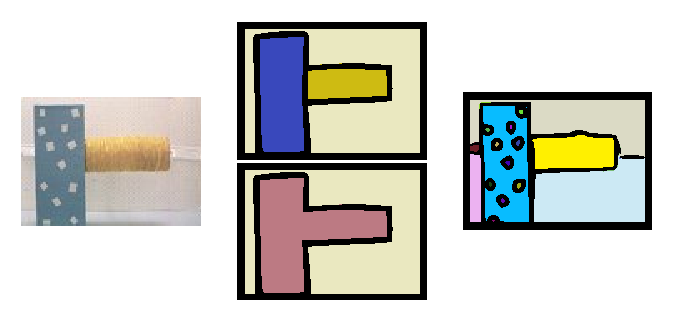
\includegraphics[width=0.75\columnwidth]{fig-seg}}

\caption{
%
Image segmentation and object segregation are different.  On the left,
there is a simple scenario, taken from \citeasnoun{needham01object}
(not quite the right image),
showing a rectangle attached to a yellow tube.  Two 
plausible ways to segregate this scene are shown in the middle,
depending on whether the tube and rectangle make up a single 
object.
For
comparison, automatically acquired boundaries are shown on the right,
produced using the algorithm in
\citeasnoun{felzenszwalb04efficient}. 
In image segmentation, the goal is to
produce regions that correspond to whole objects (such as the yellow
tube) or at least to object parts (such all the blue rectangle and all
the small white patches on its surface, and various parts of the
background).  Ideally, regions that extend across object boundaries
are avoided.  Then, higher-level processes need only consider merging
regions (of which there are a relatively small number) rather than
splitting regions (which requires a return to pixel-level
considerations).  
%
%
}

\label{fig:image-segmentation}

\end{figure}



In psychology, the human ability to divide a scene into a set of
discrete objects is termed ``object segregation.''  
In computer vision and robotics, there are algorithms with 
similar goals.  In practice, automatic object segregation
in unconstrained environments is not currently possible.
%
Progress has been made on a related, less ambitious problem
called ``image segmentation''.  The goal of image segmentation
is to divide an image of a scene into a set of discrete
regions, where each region corresponds to an object or 
an object part.  The distinction between this and 
segmentation is made clear in Figure~\ref{fig:image-segmentation}.
%
Image segmentation will typically produce more regions than there are
objects.  The idea is that those ``summary'' regions could then be
merged by more informed, higher level processing (although successful
algorithms for such higher level processing do not actually currently
exist for unconstrained environments).  Regions designed to be
used this way are also called ``superpixels''.
%
They can be produced by bottom-up processes that look for 
similarily in color and texture.  We give an example algorithm later
in this section.
%

For humans, visual experience is continuous, and comes from our two
eyes.  Image segmentation can be generalized to video sequences, and
to input from multiple view-points.  Real-time, robotic
implementations of image segmentation are primitive compared to
state-of-the-art off-line segmentation algorithms, and focus on simple
cases, such as colorful or moving objects.
%
However, robotic work is potentially well suited to addressing the
parts of object segregation that have been omitted from image
segmentation: specifically, the role of {\em experience} over
various time-scales.  Object boundaries are revealed in some
circumstances and obscured in others; how do we propogate this
information?  We can ask this over short time-scales, within
a working session, or over longer time-scales and ranges
of experiences.

We look at the role of experience in infants' object 
segregation skills, and work to factor experience into 
image segmentation for machine vision.


\subsection{Development of infants' object segregation skills}

It is clear that human infants learn generic principles for making
educated guesses about which surfaces belong together as part of the
same unit and which do not.  By 4 to 5 months of age, infants can
parse simple displays into units based on something like static
gestalt principles, probably some subset of these (e.g. \citeasnoun{needham98infants,needham00improvements}).

Similar results have been obtained by researchers using partly
occluded objects (Johnson--+ display??)

Initial studies indicated that infants used some collection of
features to parse the displays \cite{needham98infants,needham97object,needham98effects}; subsequent studies suggested that object shape is the key
feature that young infants use to identify boundaries between adjacent
objects \cite{needham99role}.

These principles may lead to many incorrect parsings, but they will
also provide reasonable best guess interpretations of uniform objects
in complex displays.  


Supporting a differentiation view of the development of
generalization, Bahrick's findings suggest that young (i.e.,
2-month-old) infants are more likely to generalize farther from the
specific experiences they received than infants just a few months
older (get citation).  This finding suggests that experience might
serve to initially narrow and then extend the range of stimuli over
which young children will generalize.


Infants do not come prepared to segregate objects into units that
adults would consider meaningful.  Rather, infants learn how object
features can be used to predict object boundaries.  More than twenty
years ago, \citeasnoun{kellman83perception} suggested that infants may be born
with knowledge about solid, three-dimensional objects and that this
knowledge could help them interpret portions of a moving object as
connected to other portions that were moving in unison.  However, this
assertion was put to the test by Slater and his colleagues (is this
\citeasnoun{slater90newborn}?), a test that resulted in a new conception of
the neonate's visual world.  Rather than interpreting common motion as
a cue to object unity, they interpreted the visible portions of a
partly occluded object as clearly separate from each other, even when
undergoing common motion.  This finding was important because it
revealed one way in which learning likely changes how infants
interpret their visual world.


Although adjacent objects present a very similar kind of perceptual
problem (are these surfaces connected or not), the critical components
of success might be quite different.  Early work with adjacent objects
indicated that at 3 months of age, infants tend to group all touching
surfaces into a single unit \cite{kestenbaum87perception}.
Subsequent experiments have revealed that soon after this point in
development, infants begin to analyze the perceptual differences
between adjacent surfaces and segregate surfaces with different
features (but not those with similar features) into separate units
(Needham 2000).  Although infants can use the boundary seam between
two objects as a source of information about the likely separation
between them (Kaufman \& Needham, submitted), other work comparing
boundary-occluded and fully visible versions of the same displays
suggests that boundary information is not the only information infants
use to parse the objects in a display (Needham, 1998).  

Infants also use information about specific objects or
classes of objects to guide their judgement.  
NEEDHAM, CANTLON, \& ORMSBEE 2005 (age: 8.5 months).


It might be that extensive amounts of experience are required to
`train up' this system.  However, it might also be that infants learn
on the basis of relatively few exposures to key events (Baillargeon,
1999).  This possibility was investigated within the context of object
segregation by asking how infants' parsing of a display would be
altered by a brief prior exposure to one of the objects in the test
display.



\subsection{Specific instances of experience affecting infants' segregation judgements}

In this paradigm, a test display was used that was ambiguous to
4.5-month-old infants who had no prior experience with the display.
Prior experience was given that would help disambiguate the display
for infants.  This experience consisted of a brief prior exposure
(visual only) to a portion of the test display.  If infants used this
prior experience to help them parse the test display, they should see
the display as two separate objects and look relaibly longer when they
moved as a whole than when they move separately.  Alternately, if the
prior experience was ineffective in altering infants'
interpretation of the display, they should look about equally at the
display, just as the infants in the initial study with no particular
prior experience did \cite{needham98effects}.  Prior experiences
with either portion of the test display were effective in facilitating
infants' parsing of the test display.  

However, when we introduced changes between the box seen during
familiarization and that seen as part of the test display, an
unexpected pattern emerged.  Nearly any change in the object's
features introduced between familiarization and test prevented infants
from benefitting from this prior experience.  So, even when infants
saw a blue box with yellow squares prior to testing, and the box used
in testing had white squares but was otherwise identical, they did not
apply this prior experience to the parsing of the test display.
However, infants did benefit from the prior exposure when it was not
in the features of the object but rather in its orientation 
 \cite{needham01object}.  
A change in the orientation of the box from horizontally to
vertically oriented led to the facilitation in parsing seen in some
prior experiments.  Thus, infants even as young as 4.5- to 5-months of
age know that to probe whether they have seen an object before, they
must attend to the object's features rather than its spatial
orientation \cite{needham01object}.

These results also support two additional conclusions.  First,
infants' object representations include detailed information
about the object's features.  Because infants'
application of their prior experience to the parsing of the test
display was so dependent on something close to an exact match between
the features, one much conclude that a highly detailed representation
is formed on the initial exposure and maintained during the
inter-trial-interval.  Because these features are remembered and used
in the absence of the initial item and in the presence of a different
item, this is strong evidence for infants' representational
abilities.  Secondly, 4.5-month-old infants are conservative
generalizers -- they do not extend information from one object to
another very readily.  But would they extend information from a {\bf group}
of objects to a new object that is a member of that group?


\subsection{Generalization of knowledge gained from experience}

This question was investigated by \citeasnoun{needham05infants}
in a study using the same test display and a similar procedure as in
\citeasnoun{needham01object}.  Infants were given prior experiences with collections
of objects, no one of which was an effective cue to the composition of
the test display when seen prior to testing.  A set of three similar
objects seen simultaneously prior to test did facilitate 4.5-month-old
infants segregation of the test display.  But no subset of these three
objects seen prior to testing facilitated infants' segregation of the
test display.  Also, not just any three objects functioned in this way
-- sets that had no variation within them or that were too different
from the relevant test item provided no facilitation.  Thus,
experience with multiple objects that are varied but that are similar
to the target item is important to infants' transfer of their
experience to the target display.



This finding was brought into the ``real'' world by investigating
infants' parsing of a test display consisting of a novel key
ring (Needham et al., submitted; see Figure X).  According to a strict
application of organizational principles using object features, the
display should be seen as composed of (at least) two separate
objects -- the keys on one side of the screen and the separate
ring on the other side.  However, to the extent that infants recognize
the display as a member of a familiar category -- key
rings -- they should group the keys and ring into a single unit
that should move as a whole.  Our findings indicate that by 8.5 months
of age, infants parse the display into a single unit, expecting the
keys and ring to move together.  Younger infants do not see the
display as a single unit, and instead parse the keys and ring into
separate units.  Infants of both ages parsed an altered display, in
which the identifiable portions of the key ring were hidden by
patterned covers, as composed of two separate units.  Together, these
findings provide evidence that the studies of controlled prior
exposure described in the previous section are consistent with the
process as it occurs under natural circumstances.  Infants'
ordinary experiences present them with multiple similar exemplars of
key rings, and these exposures build a representation that can then be
applied to novel (and yet similar) instances of the key ring category,
altering the interpretation that would come from featurally-based
principles alone.




\subsection{Role of behavior in the development of object segregations skills}

Evidence from of one set of studies reveals that young
infants' difficulty in collecting the relevant information
from visual displays may limit their success in these tasks (Johnson \&
Aslin 1995, \cite{johnson96perception}, then Johnson's eye tracking stuff
\cite{johnson04where} showing
that infants who look to the other side of the occluder, sampling
information from both sides of it, are the ones who perceive the
object parts as connected.  So, eye movements are an important factor
in this picture)

The changes in perception described throughout this section
do not occur in a vaccuum but rather in a
child who is also experiencing a range of other develomental changes.
One of these changes occurs in object
exploration -- infants' visual, oral, and manual
investigation of objects are showing huge improvements during this
same time period \cite{rochat89object}.  Relations between infants'
tendency to explore objects more or less actively and their accurate
parsing of an object display has been shown \cite{needham00improvements}, paving
the way for future studies of connections between object exploration
and object perception.





\begin{figure}[t]

\centerline{
\includegraphics[width=0.3\columnwidth]{cat}
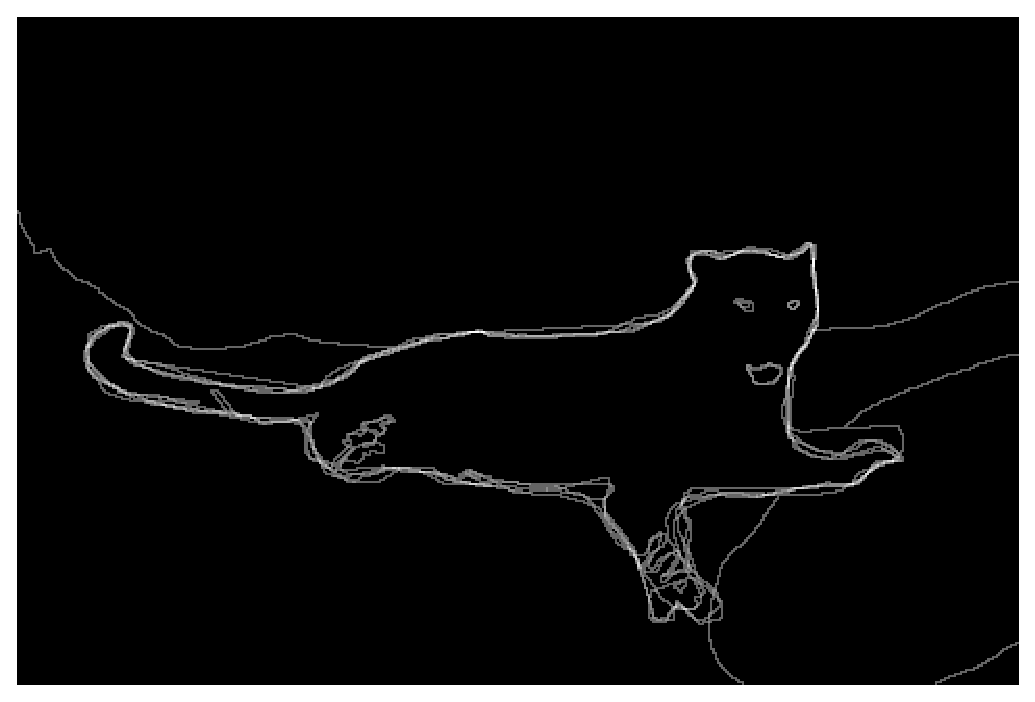
\includegraphics[width=0.3\columnwidth]{cat-human}
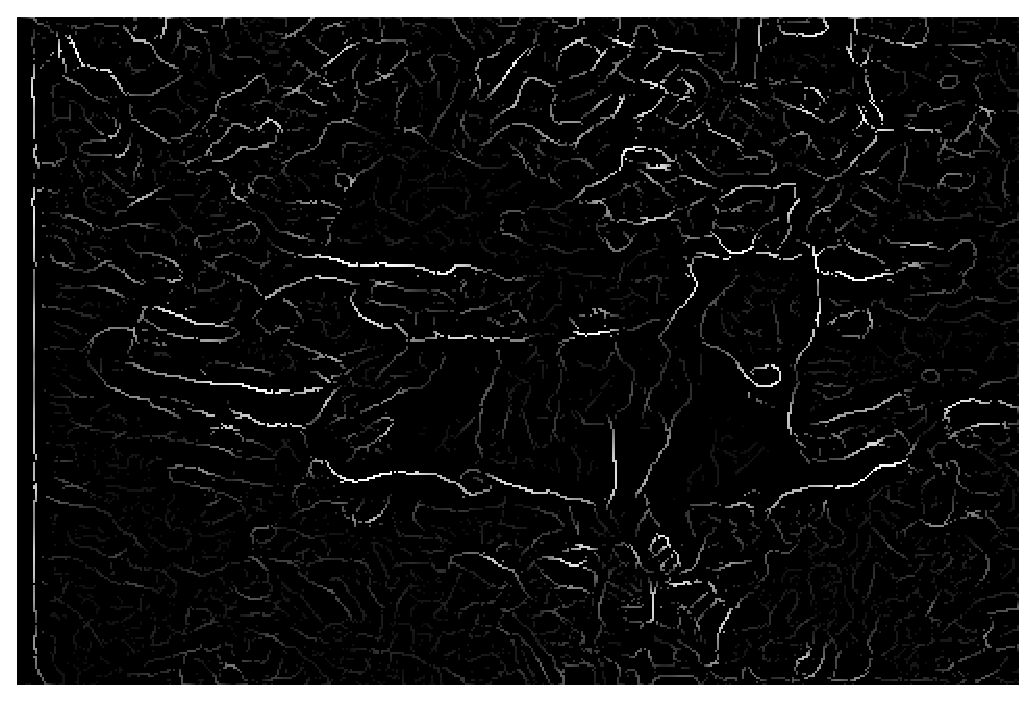
\includegraphics[width=0.3\columnwidth]{cat-machine}
}

\caption{
From [Martin et al].  Bottom-up segmentation is hard.
Image (left).  Human-labelled boundaries (middle).
Best machine segmentation of a set of algorithms (right).
}

\label{fig:segmentation-is-hard}

\end{figure}



\subsection{Object segregration in computer vision}

Object segregation is a problem of deep interest to researchers in
computer vision and robotics.  Many algorithms exist for many variants
of the problem.  
Of course, none of them even comes close to human (or
infant) performance.  
Spelke wrote in 1990:

\begin{quote}

... the ability to organize unexpected, cluttered, and
changing arrays into objects is mysterious: so mysterious
that no existing mechanical vision system can accomplish this task
in any general manner.
\cite{spelke90principles}

\end{quote}

\noindent
This is still true today.
For example, Figure~\ref{fig:segmentation-is-hard} shows the
output of a start-of-the-art algorithm for finding boundaries in images
\cite{martin04learning} compared with human performance.  This is
admittedly a particularly difficult case, but it is clear that 
a remains to
be done.


The segregation problem has been formalized in various ways.  Here is
a typical formalism (which is in fact used for many problems, not just
segregation).  There is an input image, $X$, which is a view of the
world from a camera, represented as a matrix of {\em pixels}.  Each
pixel is a simple real number representing gray-level, or a vector
representing color in RGB.
%
There is an output matrix, $Y$, where each pixel is replaced by
a {\em label}, a simple integer.  Pixels corresponding to the 
same label are considered to belong to the same region.

We can construct an {\em energy function} that evaluates the quality
of the labelling in terms of the input.  This function is designed so
that by minimizing it (by changing our choice of labelling, $Y$), we
get good results.  The energy function can be broken into two
parts:

\begin{displaymath}
%
E(X,Y) = E_{smooth}(Y) + E_{data}(X,Y)
%
\end{displaymath}

$E_{smooth}$ measures how well our labelling matches the
expectation that neighboring pixels should generally have the
same label (belong to the same region).
As far as this term is concerned, the smoother the better -- there is
a cost for neighboring pixels being assigned different labels.
$E_{data}$ measures conflicts between the labelling and the data (for
example, assigning equal labels to pixels with very different
appearance.

Particular forms of the energy function admit of efficient 
approximate solutions, and have been the topic of much research.
%
The energy function is usually {\em local} -- terms are computed 
based on comparisons between small neighborhoods of pixels.
%
This formalization works well with grouping based on local
cues -- similarity in brightness, color, and some forms of texture.
It is less suited to ``shape'' cues.


Object boundaries are much more difficult to detect reliably than might be 
expected from introspection.
Statistics learned from data has been shown to be useful
\cite{konishi03statistical}.  Large databases of 
human-labelled boundaries are being collected and
used to train better systems
\cite{martin04learning}.
%
Such databases are extremely time-consuming to produce.
%
\citeasnoun{ross05learning} developed a system that performs
segmentation based on static cues (color, texture, brightness)
using statistics learned from motion segmentation.
In principle, motion is a very powerful cue for
segmentation; certainly that is the case for infants
[CITE].
%
Progress is being made on motion segmentation, both 
in improving its accuracy and increasing its efficiency
 \cite{cremers05motion,fowlkes04spectral,smith03motion,smith04layered}.
%
Currently, accurate motion segmentation is 
computationally challenging in unconstrained environments.


\subsection{Object segregration in robotics}

For object segregation in robotics, the biggest challenge is real-time
operation~-- many state-of-the-art segmentation algorithms are
unacceptably slow.  On the other hand, robots have two very
advantageous properties.  
%
The first is
{\em locality}~-- a robot exists at a certain time and place, and the
set of objects it must work with at any moment is bounded.  
%
The second is
{\em continuity}~-- a robot has a longer term relationship with
the objects embedded in its sensors than, for example, a car 
detector searching through images on the web.
%
These conditions encourage approaches to object segregation
that are experience-driven.
%
The key to such approaches is to find
opportunities in the robot's experience where the
true boundary of an object can be reliably inferred,
and then determine correlates of the boundary that 
are available more generally.
%
For example, \citeasnoun{fitzpatrick03grounding} used
a very specific condition (objects being hit by
people or the robot itself) to extract good
motion-based object boundaries; surface features
of the object could then be used to segregate that
object out in static presentations \cite{fitzpatrick03object}.
\citeasnoun{arsenio05exploiting} used rhythmic motion
of objects to segment their boundaries both in
visually and acoustically.
%
Arsenio (CITE THESIS) developed a set of techniques for acquiring all
sorts of segmentations.  Some methods work for small, grasp-size
objects, others work for large background objects like walls or
tables.





\begin{figure}[t]

\centerline{

\includegraphics[width=0.75\columnwidth]{fig-robot}
}

\caption{
%
Object segregation based on specific object experience.  The robot
detects object boundaries experimentally \cite{fitzpatrick03object}.
It searches for good features of the object that contrast with other
objects, and that are stable with respect to certain geometric
transformations.  These features are then used to jointly detect
and segment the object in future views.  Left: the robot.
Middle: segmentations of an object derived opportunistically
from experience.  Right: the robot's perspective on a scene 
containing the object on a table.  The object is correctly segmented;
the table is completely ignored.
%
}

\label{fig:robot}

\end{figure}



These systems are limited in how information from experience can be
generalized.  In \citeasnoun{fitzpatrick03object}, for example,
information is either pooled across all contexts (in the case of edge
appearance modeling) or intended to be specific to one particular
object.  There is no notion of object category.
%
In this respect, Needham's results on generalizations are
very interesting, in possibly pointing a way forward.


\subsection{Discussion of available cues and their reliability}

Using color and texture features is perhaps limiting, since they
are relatively accidental.  Infants seem to ignore them for
certain purposes [CITE].
%
Physical boundaries are functions of object shape.  But object shape
is difficult to recover in natural scenes.
%
One correlate of shape is object contour.  In a comparision between
contour-based and appearance-based methods for object categorization
\cite{leibe03analyzing}, shape-based cues are shown to be
particularly useful for categorization.
Ditto \cite{lecun04learning}.
For specific tasks, color/texture can be useful, but for 
generic tasks they are a distraction.

Biologically inspired mechanisms are competitive:
Serre's model for recognition \cite{serre05object}.


Discuss value of cues in terms of information content (how many bits),
accessibility (how hard is it to actually estimate those bits
correctly), constancy over different timescales and variations.

Luminance, color, texture, motion, shape, location, seams, stereo,
shadow.

For segregation and (a little bit) for recognition.

Pending:

\cite{swain91color}.

\cite{schiele00recognition}.

\cite{lowe04distinctive}

\cite{felzenszwalb04efficient}

maturation v experience \cite{quinn05learning}.

In figure, using \cite{felzenszwalb04efficient}.

\cite{gibson88exploratory}

\cite{spelke90principles}

\cite{martin01database}

The Torralba-led contextual approach.


shadows and interreflections for object contact
\cite{madison01use}.


Stereo review -- depth maps, making progress
\cite{scharstein02taxonomy}

theoretically, more info at corners \cite{feldman05information}

connectionist model
\cite{mareschal02learning} --

\begin{quote}

For infants younger than 6 months, common motion of surfaces that lead
behind an occluder is both necessary and sufficient to specify their
unity. Only after 6 months do infants utilize additional sources of
information for unity, such as surface appearance, and edge and
surface orientation. \cite{mareschal02learning}

\end{quote}


Wilcox on the why \cite{wilcox99object}.  Maybe don't get
``sufficient contrastive evidence within the context of
occlusion events''.


Also of interest:

\begin{quote}

In contrast, infants first demonstrate color constancy around 4-5
months of age, and then only under limited conditions ( Dannemiller
and Dannemiller).

Finally, because form features are amodal - they can be
experienced visually, orally, or haptically - they may be more
salient to young infants.

\end{quote}

Color constancy in 4-month olds: \cite{dannemiller87test} -- some 
limitations.

Nifty: not age at which feature is detectable, but the actual
info it carries, that affects at what age it gets used for
individuation -- luminance test \cite{woods05infants}.

Infants' formation and use of categories to segregate objects 
\cite{needham05infants}.

Feature priming -- \cite{wilcox04priming}


stacked objects sharing a boundary are harder
to segregate than the same two objects
side by side?  attrib to needham by xu,
paintbrush/keyring.


texture hint \cite{johnson96perception}?

depth placement and contour ownership?

\begin{quote}

Spelke noted that any mechanism for segmenting the visual array
into objects must ascertain the boundaries of adjacent objects,
the complete shapes of partly occluded objects, and the continued
existence of objects that are no longer visible.
(Johnson 1996 quoting Spelke 1990 - get original)

\end{quote}

Relatable edges: can be connected with a smooth monotic
curve behind occluder.

Including and excluding ``perceptual completion.''

Interesting developmental progressions, e.g. of perception
of transparency: \cite{johnson00infants}


Some quick learning shown via eye movements \cite{johnson03development}.


There is a difference of concerns.  In infant research, have
at least two instances of scenarios where infant has
plastic perception.

In fact habituation paradigm requires a form of short-term
plasticity. 


\cite{prechtl01role} influence of vision on early motor 
development.

\subsection{Active vision}

\cite{bajcsy88active,aloimonos87active,ballard91animate}

driven by uncertainty \cite{whaite97autonomous}, 
extensions in SLAM.

Computational color constancy isn't that great
\cite{barnard02comparison}.

<<<<<<< section-segregation.tex
More motion segmentation \cite{smith04layered}...

Habituation -- how does it really work \cite{sirois02models}.
Attraction to familiar; attraction to novelty.
How to build such a system?

sensorimotor account \cite{oregan01sensorimotor};
infant representation a challenge.  Controversy.



\begin{verbatim}

Points: mature segmentation is knowledge intensive.
Clear developmental progression in infants.
Related to individuation.
Experience influences segmentation, even on short time-scales.
Tied into meaning? (action/needham,tomasello).
Surface features relatively untrusted; implies open, changing 
environment (untrustworthy lighting etc).

Short time-scale improvements in segmentation completely
absent in computer vision.

But what about action?

Current segmentation techniques are just
the very beginning -- much more functionality required.

Continous experience?  Adv. of continuity, recurrence.

\end{verbatim}


=======
Habituation -- how does it really work \cite{sirois02models}.
Attraction to familiar; attraction to novelty.
How to build such a system?

sensorimotor account \cite{oregan01sensorimotor};
infant representation a challenge.  Controversy.

Image parsing \cite{tu05image}.

Other long term learning -- surveillance \cite{stauffer00learning}.




\section{Intermodal integration}


Events in the world have complicated effects, and can often have
a detectable impact on many of our senses.  Determining which
components of what we sense are due to the same event can be a 
difficult judgement to make.  It is a useful exercise, though.
(List reasons why)


\cite{lewkowicz00development}
\cite{lewkowicz80crossmodal}
\cite{lewkowicz04learning}
\cite{bahrick04development}
\cite{hernandez01development}
\cite{bahrick03development}
\cite{bahrick00intersensory}
\cite{gibson86ecological}
\cite{prince05synching}

In robotics: and in speech recognition / computer vision, there's
a lot of interest in matching lip movement with speech sounds - 
both to identify which of a set of people is speaking, and to
improve recognition performance by adding extra features.

Lorenzo suggests: tactile discrimination of objects, babybot work,
although not cross-modal.

Most events have components that are accessible through different
senses: A bouncing ball can be seen as well as heard; the position of
the observer's own hand can be seen and felt as it moves through the
visual field.  Although these perceptual experiences are clearly
separate from each other, composing separate `channels', we also
recognize meaningful correspondences between the input from these
channels.  How this is accomplished is not entirely clear.  Different
approaches to the development of intermodal perception posit that
infants' sensory experiences are (a) unified at birth and must be
differentiated from each other over development, or (b) separated at
birth and must be linked through repeated pairings. Although the time
frame over which either of these processes would occur has not been
well defined, research findings do suggest that intermodal
correspondences are detected early in development.

On what basis to infants detect these correspondences?  Some of the
earliest work on this topic revealed that even newborn infants look
for the source of a sound (Butterworth \& Castillo, 1976) and by 4
months of age have specific expectations about what they should see
when they find the source of the sound (Spelke, 1976).  More recent
investigations of infants' auditory-visual correspondences have
identified important roles for synchrony and other amodal properties
of objects -- properties that can be detected across multiple
perceptual modalities.  An impact (e.g., a ball bouncing) provides
amodal information because the sound of the ball hitting the surface
is coincident with a sudden change in direction of the ball's path of
motion.  Some researchers have argued (Bahrick, XXXX) that detection
and use of amodal object properties serves to bootstrap the use of
more idiosyncratic properties (e.g., the kind of sound made by an
object when it hits a surface).

A special case of visual-auditory intermodal perception is speech
perception.  We know that in adult humans, auditory and visual
information combine to create the speech sounds we hear (as evidenced
in the McGurk effect; McGurk \& McDonald (1976)).  Evidence for the
McGurk effect has also been found in infants as young as 5 months of
age (Johnson, Rosenblum, \& Schmuckler (1995).  Young infants are able
to match the visual and auditory components of one particular speech
sound (e.g., they match an open mouthshape to the ``Ah'' sound and a
wide flat mouthshape to the ``Ee'' sound -- Kuhl \& Meltzoff, 1982).
Detection of these multimodal correspondences facilitate infants'
identification of the appropriate speaker visually once the auditory
information is attended.

Movement of an object while a certain vowel sound was presented
facilitated infants' learning of the arbitrary object/sound pairing.
Thus this multimodal information that can be introduced into the
linguistic setting facilitates infants' learning of the arbitrary
connections between sounds and objects.

Multimodal motherese -- Parents tend to use new words in synchrony
with object motion, especially when their infants are younger and may
benefit more from help in attending to or understanding the referent
of the word (Gogate, Bahrick, \& Watson, 2000)



Although more work has been generated by the study of visual-auditory
relations in events, other modalities also offer this redundant
information.

Bushnell magic box study (1985, I think) -- infants reached into a box
that was created in such a way that what they saw inside the box
through a window did not match what they felt when they reached in.
10-month-olds manipulated for longer when there was a mismatch than
when there was a match in vision and haptic



Streri and Spelke did a series of studies a while back in which
infants were familiarized to two rings that were either rigidly
connected with a rod or loosely connected with a string.  Another
source of information available was the similarity in texture between
the two rings.  The studies were set up to see whether infants would
transfer information from the tactile modality (based on the texture
or movement information) with a visual display showing two separate
rings or rings connected as a single object.  Their results showed
that the rigic/nonrigid movements dimension was useful, but the
texture differences were not. Spelke used this as evidence in favor of
her idea that object attributes are not used but physical separations
or movements are used by babies to parse objects.  This idea is not
really endorsed anymore (as our studies and others have shown), but
these studies themselves might be of interest anyway.



Jeff Lockman has done some interesting work on the conditions under
which babies bang objects on surfaces.  He has found that babies are
sensitive to the affordances of the object in relation to the surface.
If th eobject has a rigid side and a nonrigid side, they'll turn the
object so that the rigid side faces the rigid surface and bang away.
The same is true if you put a handle on the object -- they'll match up
the rigid sides for banging.



On a more theoretical level, Bushnell \& Boudreau (1993) put forth the
claim that you can explain changes in infants' perceptual skills by
looking at what they're motorically capable of.  They discuss the
Klatzky \& Lederman Exploration Procedures and a few other examples in
some detail.  Their point about Klatzky \& Lederman was that until
babies/children are capable of producing the hand and arm movements
necessary for producing e.g., the up-and-down movements associated
with ``hefting'' thought to allow for the perception of object weight,
they're not going to perceive weight differences between objects.

Finally, I'm sure you know about Bahrick \& Lickliter's Intermodal (or
Multimodal?) Redundancy Hypothesis.  They've shown in babies and in
young animals (mostly bobwhite quail) that organisms learn better and
faster from multimodal stimulation.



The last thing I was thinking about mentioning is a little something
about affordances -- some people have distinguished between
first-order (or readily apparent, existing more in the external
object) affordances and second-order affordances that depend much more
on the observer's knowledge.  I'm not sure if that distinction would
be useful here or maybe even in the embodiment section, but I thought
I'd mention it.



%%\section{Object permanence}

%%
THIS SECTION HAS BEEN REMOVED


Objects persist across time.  How do we judge that something seen
now is what we saw before.  An incremental pathway to this...
Break it down, show nuances.


\cite{johnson02development}, where segments of a single object
visually divided by an occluder become linked perceptually in
young infants.


In robotics: not a whole lot.
In computer vision: there are various tracking algorithms
that deal with various degrees of occlusion and have varying
generality.

Lorenzo suggests Babybot work on the visual exploration of objects.


\section{The role of embodiment}


Hand regard.  Humans?  Robots?

Lorenzo suggests Babybot work on the visual exploration of objects.

Recent theories agree on the importance of the body to determine the emergence of intelligence and cognition in biological systems. 
From a computational point of view it is impossible to ignore the interaction between the body and the environment that leads to the formation of the sensory information reaching the brain. 
The morphology of the body affects perception in numerous ways. In primates, for example, the visual information that reaches the visual cortex has a non-uniform distribution, due to the peculiar arrangement and size of the photoreceptors in the retina. In many species the outer ears and the head filter the sound in a way that facilitate auditory localization. The intrinsic elasticity of muscles allows for a better adaptation of the limbs during interaction with the environment.
From a developmental point of view the interaction between the body and the environment is considered paramount for the correct perceptual and cognitive development of infants. 
Through the body the brain performs actions aimed to explore the environment and collect information about its properties and rules. For example through manipulation infants have direct control on the exploration of objects. When an infants holds an object, its exploration lasts longer and reveals information about weight and shape through senses like touch and proprioception. More articulated expolarative actions can bring about other properties (the sound generated from collisions, the way the object behaves when pushed and so on).

In robotics we have the possibility to study these aspects and their implications on the realization of artificial systems. Robots like humans can exploit the physical interaction with the environment to enrich and control their sensorial experience. In one experiment for example we have shown that by grasping object a robot can exploit tactile information to distinguish object of different shape, a task that would be much more difficult if performed visually.
However these abilities do not come for free. In order for the exploration of the environment to be meaningful and safe the robot must first learn how to control its body. It is perhaps not a coincidence that, in fact, motor and perceptual abilities develop together in infants. Proper control of at least the head, the arm and the hand is required before infants can reliably and repetitively engage in interaction with objects. Motor control is challenging especially when it involves the physical interaction between the robot and the world.

Exploiting actions for learning and perception requires the ability to match an action with the agent that caused it (sense of agency, Jeannerod 2002). The sense of agency gives humans the sense of ownership of their actions and implies the existence of an internal representation of the body. The experiments by Graziano and Graziano and colleagues (cite) support the existence of a representation of the arm in the premotor cortex of the primate brain. Rochat and Striano (Rochat and Striano 2000) showed that 5 months-old infants are able to recognize their own legs moving on a mirror from those of another infant. It is believed that to develop this ability infants exploit correlations across different sensorial channels (combined double touch/correlation between proprioception and vision), [although some sort of eye-hand coordination is already present at birth (Van der Meer et al. 1995)]. During development infants learn to recognize their body and to distinguish it from other entities in the environment (other people or objects). 

Inspired by these observations, roboticists have begun to investigate the problem of self-recognition in robotics (cite Yoshikawa/Metta Fitzpatrick/Natale). In the work of Yoshikawa (Yoshikawa 2003 check and cite also Yoshikawa 2004) the rationale is that for any given posture the body of the robot is invariant with respect to the rest of the world. Correlation between the visual information and the proprioceptive feedback representing different posture can be learnt by a neural network to predict the position of the arms in the visual field. In the work of Fitzpatrick and Metta, and later Natale actions are instead used to generate visual motion with a known pattern. Similarities in the proprioceptive and visual flow are searched to visually identify the hand of the robot. Periodicity in this case enhance and simplify the identification. As a result of this process the robot learns a multimodal representation of its hand that allows a robust identification in the visual field.

In our experience with robots the body schema (in our case applied only to the arm) proved useful because it allows the robot to identify the hand in the visual field and direct the gaze to fixate it. The ability to direct the attention of the robot towards the hand is particularly helpful during learning. In an experiment we showed how this ability allows the robot to learn a visual model of the object it manages to grasp by simply inspecting the hand when touch is detected on the palm. In other situations the same behavior could allow the robot to direct the gaze to the hand if something unexpected touches it. Eye-hand coordination seems thus important to establish a link between different sensory channels like touch and vision.

\section{A common model?}


Can we make some kind of common model?



%\section{Results}

%\input{section-result}



\section{Conclusions}


%% Humanoid robots are improving mechanically by leaps and bounds.
%% Stable bipedal walking (at least on flat surfaces) is now a
%% commonplace, with running and jumping on the way.  There are
%% many, many problems remaining, but it is accurate to say that
%% there has been real progress mechanically.

%% But there are some danger signs.  In robot demonstrations today,
%% you're much more likely to see synchronized dancing, gesturing, and
%% talking than any physical interaction with objects.  Robot hands and
%% arms are currently rather limited mechanically, but more importantly
%% the {\em perceptual} component of manipulation is very hard, unless we
%% constrain the environment greatly.  And while in locomotion
%% constraining the floor to be flat is not so limiting, in manipulation
%% the corresponding constraint is for the object to be of a particular
%% shape, orientation, location, etc., which is much more limiting.

In the field of humanoid robotics, researchers have a special respect
and admiration for the abilities of infants.  They watch their newborn
children with particular interest, and their spouses have to
constantly be alert for the tell-tale signs of them running an ad-hoc
experiment.  It can be depressing to compare the outcome of a 
five-year, multi-million-euro/dollar/yen project with what an
infant can do after four months.  Infants are so clearly doing what
we want to robots to do; is there any way to learn from research
on infant development?
Conversely, can infant development research be illuminated by
the struggles faced by robotics, perhaps pointing out fundamental
perceptual difficulties taken for granted?
%
%
Is there a way to create a model of development which applies both to infants
and robots?
%
It seems possible that similar sensorial constraints and opportunities
will mold both the unfolding of an infant's sensitivities to
different cues, and the organization of the set of algorithms used by
robots to achieve sophisticated perception.
%
So, at least at the level of identifying ``key events'' and mutually
reinforcing cues, a shared model is possible.
%
%For infants, this would be a theory of development, another way to
%express current theories.
%
%For robots, this would be an engineering tool, a guide to
%construction.
%
%On the infant side, empirical results would change, correct, and expand
%the model.  On the robot side, construction effort would do the same.
%
%Of course, the results could diverge, but at least they are 
%comparable, and those interested in truly humanoid robots would
%work to stay synchronized.
%
Of course, there is a lot that would not fit in the model, and this is
as it should be.  It would be solely concerned with the class of 
functional, information-driven constraints.
%
We have not in this paper developed such a model; that would be
premature.  We have at identified some points of connection that could
grow into much more.  We hope the paper will serve as one more link in
the growing contact between the fields.

%% loose threads
%\nocite{kirkham02visual}
%\nocite{johnson05building}
%\nocite{diamond05not}



%% Pending: Something about active vision?

%\nocite{bajcsy88active,aloimonos87active,ballard91animate}
%\nocite{whaite97autonomous} 
%\nocite{barnard02comparison}




\section*{Acknowledgements}


\section{Acknowledgments}

YARP and ICub make heavy use of software released under free and open
licenses -- thank you world.
%
The author would like to gratefully acknowledge contributions to YARP
from Radu Bogdan Rusu, Alexis Maldonado, Eric Mislivec, Christopher
Prince, Charles C. Kemp, Francesco Nori, Julio Gomes, Alexandre
Bernardino, Carlos Beltran, Jonas Ruesch, Assif Mirza, Hatice
Kose-Bagci, Jose Gaspar, Claudio Castellini, Michael Bucko, Nelson
Gon\c calves, Marco Barbosa, Tomassino Ferrauto, Boris Duran, Mattia
Castelnovi, and Alessandro Scalzo (if we missed anyone, plese let us
know).  We'd also like to thank contributors to the ICub project.
%
The authors were supported by European Union
grant RobotCub (IST-2004-004370).







%  Generate ``References'' here.

\nocite{natale05developmental}
\nocite{arsenio05exploiting}
\bibliographystyle{sab}
\bibliography{main}


%%\section*{Scrapyard}

%%
%% put text you don't know what to do with here

\section{SCRAPYARD - to be deleted probably}


\subsection*{YARP Network Scraps}

Not localization friendly, English bias at a quite low level.
Probably localization would not be practical at the network
protocol level.  Also approach to character encoding is
primitive and ad-hoc; no guarantee that encoded data
will survive in text-mode.



YARP is a free and open source project.  Since its source code is
released under a free and open license, useful parts of it can be used
by other systems, and its operation can be studied.

YARP has a large quantity of documentation (although we always need
more).  The communication protocol it uses is documented, and can be
interfaced with without using the YARP code-base.

Beyond just documenting the communication protocol, particular attention
has been devoted to make sure that that reading and writing data to a
YARP port can be done with very little effort.  YARP ports will 
accept and make connections of any of several different forms;
for a program build without the YARP code-base, it suffices
to implement just one of those connection types in order to
get basic connectivity.  If bandwidth requirements are not
excessive, the very simplest connection type can be implemented:
a very basic text-mode protocol.


\subsection*{Software publishing}

RANT FOLLOWS

The literature of a research community both expresses its ideas, and
aids in their evolution

Published ideas are read, evaluated, and built upon

Useful advances get published

Publication of software can speed progress

Facilitates evaluating and comparing approaches

Brings new research topics into reach

Publish or perish!

REPEATED RANT FOLLOWS

As a research community, we both read and produce papers, building on
each others' work.

We also both acquire and produce software

Our software tends to die with our projects

Sad!  Software collaboration speeds things up

Research groups that all use a specific robot (Khepera, Pioneer, AIBO,
...) often form a natural software community

But each alone is a small subset of robotics

Groups developing new robots face obstacles

Differences in sensors, actuators, bodies...

Differences in processors, operating systems, libraries, frameworks,
languages, compilers...

Big barriers to software collaboration




\subsection*{Modularity}

Constant hardware flux

Parts change rapidly

Interfaces change slowly

Lots of software grew and evolved alongside the changing hardware

Parts change rapidly

Interfaces change slowly

``Modularity'' is rewarded


The way parts interact can last longer than the parts themselves

E.g. an eternal broom

replace broom head

replace broom handle


Long-lived software is like the Ship of Theseus

The mast gets replaced

The planks get replaced

Over time, everything may get replaced

In philosophy, this is a ``paradox of identity''

For us, it's just our job


The opposite of a modular system is a coupled one.

In a ``coupled'' system, changes in one part trigger changes in another.

Coupling leads to complexity

Complexity leads to confusion

Confusion leads to suffering

This is the path to the Dark Side

Robot software is notoriously hardware-specific and task-specific

Both hardware and target tasks change quickly, even within the
lifetime of one project

Our humanoid robots are far more complex than one person can build and
maintain, both in terms of hardware and software

They need to be modular



\end{document}


